% !TEX TS-program = latex


%
\documentclass[12pt]{article}

% The usual packages
\usepackage{booktabs}
\usepackage{array}
\usepackage{subcaption}

\usepackage{fullpage}
\usepackage{breakcites}
\usepackage{setspace}
\usepackage{endnotes}
\usepackage{mathtools} % for \mathclap
%\usepackage{float} % can't use with floatrow
\usepackage{amsmath}
\usepackage{amsfonts}
\usepackage{amssymb}
\usepackage{rotating}
\usepackage{longtable}
\usepackage{microtype}
\usepackage{graphicx}
\usepackage{hyperref}
%\usepackage[usenames,dvipsnames]{color}
\usepackage{url}
\usepackage{natbib}
\usepackage{framed}
\usepackage{epigraph}
\usepackage{textcomp} % for \textrightarrow
\usepackage{dcolumn}
\usepackage{nameref}
\usepackage{booktabs}
\usepackage{float}
%\restylefloat{table}
\bibpunct{(}{)}{;}{a}{}{,}


\usepackage{tabularx}
\usepackage{lscape} % For landscape orientation
\usepackage{multirow} % For multirow cells
\usepackage{array}

\usepackage{nameref}



% Set paragraph spacing the way I like
\parskip=0pt
\parindent=20pt

%\usepackage{helvet}
%\usepackage[labelfont={bf}, margin=0cm, font=small, skip=0pt]{caption}

%\newcommand\numberthis{\addtocounter{equation}{1}\tag{\theequation}}

% % Define mathematical results
% \newtheorem{lemma}{Lemma}
% \newtheorem{proposition}{Proposition}
% \newtheorem{theorem}{Theorem}
% \newtheorem{claim}{Claim}
% \newtheorem{rule0}{Rule}
% \newenvironment{proof}[1][Proof]{\begin{trivlist}
% \item[\hskip \labelsep {\bfseries #1}]}{\end{trivlist}}
% \newenvironment{definition}[1][Definition]{\begin{trivlist}
% \item[\hskip \labelsep {\bfseries #1}]}{\end{trivlist}}
% \newenvironment{example}[1][Example]{\begin{trivlist}
% \item[\hskip \labelsep {\bfseries #1}]}{\end{trivlist}}
% \newenvironment{remark}[1][Remark]{\begin{trivlist}
% \item[\hskip \labelsep {\bfseries #1}]}{\end{trivlist}}
% \DeclareMathOperator*{\argmin}{arg\,min}
% \DeclareMathOperator{\med}{med}
% \DeclareMathOperator*{\E}{\text{E}}
% \DeclareMathOperator*{\Pr}{\text{Pr}}


\usepackage{amsthm}
\usepackage{thmtools}
\usepackage{thm-restate}

\declaretheoremstyle[
  headfont=\normalfont\bfseries,
  bodyfont=\normalfont,
  notefont=\normalfont\bfseries,
  postheadspace=0.5em,
  headpunct={:},
  %qed=\qedsymbol,
  spacebelow=\medskipamount,
  spaceabove=\medskipamount,
  mdframed={
    linecolor=gray!20,
    backgroundcolor=gray!10,
    linewidth=0.5pt,
    roundcorner=5pt,
    innertopmargin=5pt,
    innerbottommargin=5pt,
    innerrightmargin=5pt,
    innerleftmargin=5pt
  }
]{mytheoremstyle}

% Declare the rule environment using the custom style
\declaretheorem[name=Rule, style=mytheoremstyle]{rule0}

% A special command to create line break in table cells
\newcommand{\specialcell}[2][c]{%
 \begin{tabular}[#1]{@{}c@{}}#2\end{tabular}}

%% Set up lists the way I like
% Redefine the first level
\renewcommand{\theenumi}{\arabic{enumi}.}
\renewcommand{\labelenumi}{\theenumi}
% Redefine the second level
\renewcommand{\theenumii}{\alph{enumii}.}
\renewcommand{\labelenumii}{\theenumii}
% Redefine the third level
\renewcommand{\theenumiii}{\roman{enumiii}.}
\renewcommand{\labelenumiii}{\theenumiii}
% Redefine the fourth level
\renewcommand{\theenumiv}{\Alph{enumiv}.}
\renewcommand{\labelenumiv}{\theenumiv}
% Eliminate spacing around lists
\usepackage{enumitem}
\setlist{nolistsep}

% Create footnote command so that my name
% has an asterisk rather than a one.
\long\def\symbolfootnote[#1]#2{\begingroup%
\def\thefootnote{\fnsymbol{footnote}}\footnote[#1]{#2}\endgroup}
%\usepackage{footmisc}
%\renewcommand{\thefootnote}{\symbolfootnote{footnote}}

% Create the colors I want
\usepackage{color, xcolor}
\definecolor{color1}{RGB}{217,95,2}  % orange
\definecolor{color2}{RGB}{27,158,119}  % green
\definecolor{color3}{RGB}{117,112,179}  % purple


% set up pdf
\hypersetup{
pdftitle={}, % title
pdfauthor={Carlisle Rainey}, % author
pdfkeywords={bias} {first difference} {marginal effect} {quantities of interest} {maximum likelihood}
pdfnewwindow=true, % links in new window
colorlinks=true, % false: boxed links; true: colored links
linkcolor=black, % color of internal links
citecolor=black, % color of links to bibliography
filecolor=blue, % color of file links
urlcolor=blue % color of external links
}

% section headers
%\usepackage[scaled]{helvet}
%\renewcommand\familydefault{\sfdefault}
%\usepackage[T1]{fontenc}
\usepackage{titlesec}
\titleformat{\section}
 {\normalfont\sffamily\Large\bfseries}
 {\thesection}{1em}{}
\titleformat{\subsection}
 {\normalfont\sffamily\bfseries}
 {\thesection}{1em}{}
 \titleformat{\subsubsection}
 {\normalfont\sffamily\bfseries}
 {\thesection}{1em}{}

% enable comments in pdf
\newcommand{\dtk}[1]{\textcolor{blue}{#1}}
\newcommand{\ctk}[1]{\textcolor{red}{#1}}

\begin{document}

\begin{center}

{\huge \textbf{Power Rules}\symbolfootnote[1]{This essay flows from many discussions with undergraduate and graduate students. 
In these discussions, we have thought about power as a minor extension of estimation and inference rather than power as a distinct topic. 
In this essay, I try to articulate that perspective and help researchers extend their familiarity with estimation and inference to thinking about statistical power.}
}

\vspace{0.4cm}


{\Large\textbf{Practical Statistical Power Calculations}}



\vspace{1cm}

Carlisle Rainey\symbolfootnote[2]{Carlisle Rainey is Associate Professor of Political Science, Florida State University, 540 Bellamy, Tallahassee, FL, 32306. (\href{mailto:crainey@fsu.edu}{crainey@fsu.edu}).}

\vspace{1cm}
\today 
\vspace{5mm}

Draft \textit{very much} in progress. \\
Comments welcomed! (\href{mailto:crainey@fsu.edu}{crainey@fsu.edu}) \\\vspace{2mm}
Get latest version \href{https://github.com/carlislerainey/power-rules/blob/main/power-rules.pdf}{from GitHub}.
\end{center}

\vspace{5mm}

% Abstract
{\centerline{\textbf{Abstract}}}
\begin{quote}\noindent
Recent work in political science emphasizes the importance of statistical power in political science and shows that power in political science tends to be extremely low. 
In this paper, I offer simple rules that make statistical power more approachable for substantive researchers. 
In the cases of simple treatment effects and interactions, these rules are sufficient for a complete and compelling power analysis using only paper-and-pencil. 
In other cases, these rules can provide a useful ballpark prediction before turning to specialized software or complex simulations. 
The rules allow researchers to predict statistical power using (1) features of a reference population, (2) an existing study with a similar design and outcome, and/or (3) a pilot study. 
For example, it can be helpful for readers and researchers to know that experiments have 80\% power to detect effects that are 2.5 times larger than the standard error. 
I hope these rules will lower the barrier to entry for researchers new to thinking carefully about statistical power and help researchers design powerful, informative experiments.
\end{quote}

% Add quote to first page
% \epigraph{}

%\begin{center}
%Manuscript word count:
%\end{center}

% Remove page number from first page
\thispagestyle{empty}
\newpage

% Start main text
%\newpage
\doublespace
%\onehalfspace

\setcounter{page}{1}


\section*{Introduction}

Experiments continue to grow in political science \citep{Druckman2021}, and designing an experiment requires us to either select an appropriate sample size or evaluate whether a given sample size is sufficient for our goals.\footnote{
  For example, the \emph{Journal of Politics} guidelines for registered reports notes that ``a detailed justification of the planned sample size is essential'' (accessed May 2, 2024, persistent link: \url{https://archive.md/g7YQ3}). 
  The \emph{Journal of Experimental Political Science} requires authors to ``explain how the sample size was determined and note statistical power'' (accessed May 2, 2024, persistent link: \url{https://archive.md/7nLKg}). 
  Time-sharing Experiments for the Social Sciences (TESS) notes that power analysis is ``encouraged'' (accessed May 11, 2024, persistent link: \url{https://archive.md/Xc0UY}). 
  The Civic Health and Institutions Project, a 50 States Survey, (CHIP50) notes that power analysis is ``strongly encouraged'' (accessed May 11, 2024, persistent link: \url{https://archive.md/SLpgW}). 
  The National Institutes of Health (NIH) provides several examples to ``demonstrate rigor'' and all examples include a discussion of statistical power (accessed May 11, 2024, persistent link: \url{https://archive.md/Jh9Lp}). 
  The popular OSF pre-registration template asks user to provide an explicit sample size rationale, which could include a power analysis \citep{Bowman2020}.}
Statistical power, or the chance of rejecting the null hypothesis for a given treatment effect, is a common, powerful way to select or evaluate a sample size.
The consequences of low power are increasingly understood: low power can lead to wildly overestimated treatment effects \citep{Gelman2014} and ambiguous results that are difficult to publish (e.g., \citealt{Alrababah2023}). 
Nonetheless, \cite{ArelBundock2022} argue that only about 10\% statistical tests in political science have at least 80\% power. 
Underscoring their important findings, \cite{ArelBundock2022} emphasize: ``our research community must address the problems of low power and selection on significance with institutional, methodological, and theoretical remedies.''

One apparent problem is that while political scientists understand estimation and inference for experimental data very well (e.g., least squares regression with robust standard errors), political scientists are less comfortable thinking about statistical power prior to data collection. 
This apparent discomfort is not without reason. 
Power analysis requires specialized software or tedious simulation. 
Most specialized software, such as G*Power \citep{Faul2007, Faul2009}, is designed primarily for psychologists. 
The language (e.g., Cohen's \emph{d}) and style of analysis (e.g., ANCOVA) can make the software awkward for political scientists (though of course not insurmountable).\footnote{
  For example,the power resources that the \emph{Journal of Politics} provides include links to several resources for planning sample size in experiments, but many of their resources are directed primarily at psychologists.
  }
Most importantly, political scientists tend to focus on treatment effects on the scale of the outcome (e.g., \citealt{King2000}), while psychologists are more comfortable with standardized effect sizes.\footnote{
  \cite{Lakens2022} offers a careful and thorough discussion of sample size justifications for an audience of psychologists, but (appropriately) uses terms common in psychology.
  For example, Lakens centers much of his discussion around Cohen's \emph{d}, standardized effect size used often in psychology but less often in political science.
  } 
In political science, recent conceptual work and statistical software \citep{Blair2019, Blair2023} make complex simulations to evaluate research designs more accessible, but simulation to obtain statistical power remains challenging compared to analyzing experimental data.

In this paper, I offer several simple rules for assessing statistical power. 
These rules do not require special software or simulation and are motivated from statistical analyses common in political science. 
I tightly connect the rules for statistical power to the logic of estimation and inference for experimental data in political science (least squares regression, robust standard errors, and confidence intervals).
There is tremendous value in simple, conceptual rules of thumb---the kind of rules that allow us to predict the statistical power of an experiment with paper, a pencil, and (perhaps also) a pocket calculator.\footnote{
  My own view is that paper-and-pencil calculations are valuable, for two reasons. 
  First, predicting statistical power involves a fair amount of guesswork. 
  Specialized software and simulations bring an air of exactness that does not seem to match the spirit of the task. 
  With paper-and-pencil calculations, it seems easier to remember that task is to make an informed guess. 
  Second, paper-and-pencil work constantly reminds us how inputs relate to outputs. 
  Since we are \emph{designing} experiments and have freedom to make different design choices, it can be helpful to be constantly reminded of the relationship between inputs and outputs.
  }
While specialized software and complex simulations are helpful (and essential in some cases), simple rules have several benefits: 
(1) simple rules can make statistical power accessible, rather than seem like a mystical quantity; 
(2) simple rules allow us to reason fluently about design choices; 
(3) even if we ultimately rely on a more sophisticated approach, simple rules can reduce the chance of making big errors by giving us a ballpark starting point; and
(4), in many cases, simple rules are sufficient to justify a sample size and simulations and specialized software are unnecessary. 
In this paper, I walk through several rules to predict the statistical power of an experiment. 
I explain the intuition of each rule, describe how we can use the rule to plan or evaluate a study, and give examples.

\section*{Review: The Estimation and Inference Framework}

Throughout this discussion, I assume that we use ordinary least squares and robust standard errors to estimate the treatment effect. 
I assume size-0.05, one-sided tests of directional hypotheses evaluated in practice using 90\% confidence intervals.\footnote{
  A later section describes how researchers can modify the rules for 95\% confidence intervals
}
I borrow the language of survey experiments about the experimental units as ``respondents,'' but the logic generalizes to other types of units (e.g., villages). 

Formally, I assume potential outcomes $\mathcal{Y}_{i}(1)$ if assigned to treatment and $\mathcal{Y}_{i}(0)$ if assigned to control for respondent $i$ of $N$. 
An experiment might use more than two conditions, but for the sake of the discussion below, I focus on the statistical power of a comparison of just \emph{two} of these conditions, which I call treatment and control.
For these two conditions, we want to make inferences about the treatment effect $\tau = \frac{1}{N}\sum_{i = 1}^{N}{\mathcal{Y}_{i}(1)} - \frac{1}{N}\sum_{i = 1}^{N}{\mathcal{Y}_{i}(0)}$.

To make inferences about $\tau$, we randomly assign $n_{1}$ respondents to treatment and $n_{0}$ respondents to control, where $N = \ n_{1} + n_{0}$.\footnote{
  Note that $N$ represents the \emph{total number of the respondents} in the comparison, while $n_{i}$ represents the number of respondents \emph{in condition} $i$\emph{.}
  Below, I assume equal numbers of respondents in each condition, so I let $n$ represent the number of respondents per condition, which is a convenient quantity when thinking about experimental design and statistical power.
  }
We create an indictor variable $D_{i}$ that equals 1 if the respondent is assigned to treatment and 0 if the respondent is assigned to control. 
Then we create the observed outcome $Y_{i} = \mathcal{Y}_{i}\left( D_{i} \right)$ by assigning $Y_{i}$ the potential outcome under treatment if $D_{i} = 1$ and the potential outcome under control if $D_{i} = 1$. 
Then we estimate the treatment effect using $\widehat{\tau} = \frac{1}{n_{1}}\sum_{i = 1}^{N}{{D_{i} \cdot Y}_{i}} - \frac{1}{n_{0}}\sum_{i = 1}^{N}{{\left( 1 - D_{i} \right) \cdot Y}_{i}}$, which we compute in practice using least squares estimates of the model $Y_{i} = \alpha + \tau \cdot D_{i} + \epsilon_{i}$. 
In some cases, we might increase the precision of the estimates by including variables measured pre-treatment as control variables in the regression model.


  
To estimate the sampling variance of $\widehat{\tau}$, we use Neyman's (\citeyear{Neyman1923}) conservative variance estimator $\widehat{Var}\left( \widehat{\tau} \right) = \ \frac{s_{1}^{2}}{n_{1}} + \ \frac{s_{0}^{2}}{n_{0}}$, where $s_{1}^{2}$ and $s_{0}^{2}$ represent the sample variance in the treatment and the control group, respectively. 
Then we can estimate the standard error of $\widehat{\tau}$ with ${\widehat{SE}}_{\widehat{\tau}} = \ \sqrt{\widehat{Var}\left( \widehat{\tau} \right)}$.

In practice, we use a HC2 heteroskedasticity-robust variance estimator (or a closely related variant), which \cite{Samii2012} show is equivalent to Neyman's estimator. 
For testing, \cite{Li2017} provide several additional (seemingly innocuous) regularity conditions such that a finite-sample version of the central limit theorem holds and $\left\lbrack \widehat{\tau} - \Phi_{std}^{- 1}\left( 1 - \ \frac{\alpha}{2} \right) \cdot {\widehat{SE}}_{\widehat{\tau}},\ \widehat{\tau} + \Phi_{std}^{- 1}\left( 1 - \ \frac{\alpha}{2} \right) \cdot {\widehat{SE}}_{\widehat{\tau}} \right\rbrack$ is an asymptotically conservative $\left( 1 - \ \frac{\alpha}{2} \right) \cdot 100\%\ $ confidence interval. 
We can use the 90\% confidence interval = $\left\lbrack \widehat{\tau} - 1.64 \cdot {\widehat{SE}}_{\widehat{\tau}},\ \widehat{\tau} + 1.64 \cdot {\widehat{SE}}_{\widehat{\tau}} \right\rbrack$ to conduct size-0.05 tests of directional hypotheses by rejecting a null hypotheses if and only if \emph{all} values in the 90\% confidence interval are consistent with the research hypothesis \citep{Rainey2014, McCaskey2015}.

\section*{Rules \ref{rule:power-int} and \ref{rule:power-z}: What is Statistical Power?}

In a designed experiment, we usually have a theoretically motivated research hypothesis that we would like to test. 
This research hypothesis implies a null hypothesis that we hope to reject. 
For simplicity, I assume throughout much of this paper that we hypothesize a \emph{positive} treatment effect so that $H_{R}:\tau > 0$. 
The extension to a negative treatment effect is obvious.

Imagine that we repeatedly re-randomize to treatment and control and compute $\widehat{\tau}$ for each repetition. 
Then $\widehat{\tau}$ will vary across these repeated experiments. 
We refer to the distribution of $\widehat{\tau}$ across these hypothetical
repeated experiments as the \emph{sampling distribution} of $\widehat{\tau}$. 
This sampling distribution is typically centered over the treatment effect (i.e., $\widehat{\tau}$ is unbiased or nearly so). 
Importantly, the standard deviation of the sampling distribution of $\widehat{\tau}$ is called the \emph{standard error} and ${\widehat{SE}}_{\widehat{\tau}}$ is usually a precise estimator of the standard error.

If the research hypothesis $H_{R}:\tau > 0$ is correct, then the sampling distribution of $\widehat{\tau}$ lies mostly to the right of zero. 
However, we will only claim that $\tau > 0$ if the entire 90\% confidence interval is larger than zero, or, equivalently, if $\widehat{\tau} - 1.64 \cdot \ {\widehat{SE}}_{\widehat{\tau}} > 0.$
This means that we must design our experiment so that the sampling distribution falls relatively far from zero.

We say that the statistical \emph{power} of an experiment is the chance of rejecting the null hypothesis \emph{for a particular treatment effect} $\tau$. 
For example, we say that an experiment has ``80\% power to detect a treatment effect of \underline{~~~~~}'' if
$\widehat{\tau} - 1.64 \cdot {\widehat{SE}}_{\widehat{\tau}} > 0$ in 80\% of repeated experiments.
Similarly, we say that the experiment has ``95\% power to detect a treatment effect of \underline{~~~~~}'' if the $\widehat{\tau} - 1.64\ {\widehat{SE}}_{\widehat{\tau}} > 0$ in 95\% of repeated experiments. 
By convention, 80\% power is the minimal standard for ``adequate'' statistical power \citep{Cohen1988}, but others recommend higher power, such as 95\%.\footnote{
  For example, the \textit{Journal of Politics} ``a power of at least 0.90, ideally 0.95, to detect anticipated/relevant effect sizes'' for registered reports (accessed May 3, 2024; persistent link: \url{https://archive.md/g7YQ3}). 
  \textit{Nature Human Behavior} requires that ``the a priori power must be 0.95 or higher for all proposed hypothesis tests'' for registered reports (accessed May 13, 2024; persistent link: \url{https://archive.md/xpGdj}).
  }

First, how can we compute statistical power? 
It turns out that statistical power is determined by the treatment effect and the
standard error of the estimate. 
To predict the statistical power of an experiment, we must make assumptions or ``informed guesses'' about certain quantities. 
I denote these assumed values with tilde. For example, I denote the assumed treatment effect as $\widetilde{\tau}$.\footnote{
  We have three $\tau$s floating around: the \emph{actual} treatment effect $\tau$, the treatment effect \emph{assumed for the sake of computing power} $\widetilde{\tau}$, and, the \emph{estimated} treatment effect $\widehat{\tau}$. 
  I read the tilde notation as ``assumed to predict power.'' 
  For example, I read $\widetilde{\tau}$ as ``the treatment effect assumed
  to predict power.'' 
  The tilde notation also means ``Wait!---think about this carefully, it is an assumption requiring judgment.''}
This just means ``the treatment effect we are assuming for the sake of computing statistical power.''

How can we compute the statistical power of an experiment? 
An intuitive approach uses the construction of the 90\% confidence interval. 
Recall that we will reject the null hypothesis if the lower-bound of the 90\% confidence interval falls above zero. 
The arms of the 90\% confidence interval are 1.64 standard errors wide.\footnote{
  I write ``about'' 1.64 standard errors because in practice we use the \emph{estimated} standard error, not the actual standard error. 
  However, the estimated standard error is sufficiently precise to treat
  the two interchangeably in this context.
  }
This means that we will reject the null of if the estimate of the treatment effect is larger than 1.64 standard errors. 
Thus, the power of the study is the percent of the sampling distribution that is larger than 1.64 standard errors. 
Recall that the sampling distribution is approximately normally distributed and centered over the treatment effect $\tau$ with standard deviation equal to the standard error of the estimate of $\tau$. 
Thus, computing the power is simply computing the percent of the sampling distribution above $1.64 \cdot SE$.



\begin{restatable}[Power; Most Intuitively]{rule0}{rulepowerint}
\label{rule:power-int}
Power equals $1 - \Phi(1.64 \cdot SE;\ \mu = \tau,\ \sigma = SE)$, where $\Phi(z;\ \mu,\ \sigma)$ is the normal CDF, $SE$ is the standard error of the estimated treatment effect, and $\tau$ is the treatment effect.
\end{restatable}

\noindent See \citet[92]{Gerber2012} for a similar presentation.

Dividing through by the standard error and then subtracting $\frac{\tau}{SE},$ we see that power also equals $1 - \Phi\left( 1.64 - \frac{\tau}{SE};\ \mu = 0,\ \sigma = 1 \right)$; the values of $\Phi\left(z;\ \mu = 0,\ \sigma = 1 \right)$ are provided in common \emph{z} tables, where $z = 1.64 - \frac{\tau}{SE}$. 
This allows us to compute power using the \emph{standard} normal CDF.

\begin{restatable}[Power; From a $z$ Table]{rule0}{rulepowerz}
\label{rule:power-z}
Power equals $\ 1 - \Phi_{std}\left( 1.64 - \ \frac{\tau}{SE} \right)$, where $\Phi_{std}(z)$ is the standard normal CDF (as found in a standard $z$ table), $SE$ is the standard error of the estimated treatment effect, and $\tau$ is the treatment effect.
\end{restatable}

\noindent Rule \ref{rule:power-z} allows us to connect statistical power to the familiar $z$ table in the appendices of many statistics textbooks or the \texttt{pnorm()} function in R.
But, more importantly, it drives home an important intuition---power is determined by the key ratio $\frac{\tau}{SE}$. 
To estimate power, we must make an informed assumption about the effect of interest and a good prediction of standard error of the estimate. 
Further, when we consider changes to the experimental design and the consequences for statistical power, it can be helpful to think about the numerator or the denominator of the key ratio $\frac{\tau}{SE}$: How do you make the effect as large as
possible? And how do you make the estimate as precise as possible?

\section*{What Treatment Effect Should I
Assume?}

To compute statistical power, we must assume a treatment effect. 
Statements about statistical power always have the form: ``the experiment has \underline{~~~~~}\% power \emph{to detect a treatment effect of \underline{~~~~~}.''} 
But obviously, we do not know the treatment effect with any precision, else we would not need to run the experiment. Thus, we must assume. 
\citet[6]{Lakens2022}  writes: ``The goal of an a-priori power analysis is to achieve sufficient power, given a specific \emph{assumption} of the effect size a researcher wants to detect'' [emphasis mine].

For any given experiment, there are three treatment effects worth thinking about: (1) the ``best guess'' of the effect, (2) the smallest plausible effect, and (3) the smallest substantively meaningful effect. 
\emph{By default, we should focus on the statistical power for the smallest substantively meaningful effect.}\footnote{
  Others refers to this effect as the ``smallest effect size of interest'' (SESOI) \citep{Lakens2018}, ``minimum effect of interest'' (MEI), and ``minimum meaningful effect'' (MME).
  }
However, when the smallest plausible effect is much larger than the smallest effect of substantive interest, we might compute power for the smallest plausible effect.\footnote{
  If the researchers are confident that a treatment effect is much larger than the smallest substantively meaningful effect, then they might decide it is wasteful to power their experiment for a treatment effect that is much smaller than the smallest plausible effect. 
  This strikes me as a reasonable argument.
  } 
Importantly, we must use our judgment: judgment about the substantive importance of effects, judgment about the empirical plausibility of various effects, and judgment about the relevance of each to the argument. 
As \citet[755]{Kirk1996} notes, ``researchers have an obligation to make this kind of judgment.''\footnote{
In full, \citet[755]{Kirk1996} writes:
\begin{quote}
  Researchers have an obligation to make this kind of judgment. 
  No one is in a better position than the researcher who collected and analyzed the data to decide whether or not the results are trivial. 
  It is a curious anomaly that researchers are trusted to make a variety of complex decisions in the design and execution of an experiment, but in the name of objectivity, they are not expected or even encouraged to decide whether data are practically significant.  
\end{quote}
} 

As a crude approximation, we might feel tempted to use a rule of thumb such as declaring a 0.15 SD increase in the outcome is a ``small'' effect (e.g., \citealt{Lovakov2021}). 
While rules of thumb can be useful as a starting point, they are only a first approximation---rules of thumb about ``small'' effects do not account for the question under study, so we must supplement these rules of thumb with additional arguments. 
\citet[see esp. pp. 261-263]{Lakens2018} and \citet[see esp. pp. 10-13]{Lakens2022} offer helpful further discussion of how we might choose an treatment effect of interest.

Making a thoughtful assumption about the treatment effect is perhaps the most challenging component of a power analysis. 
We are doing a study to learn about a treatment effect, so it feels uncomfortable to make declarations about the effect beforehand. 
It feels similarly awkward to divide effects into important and unimportant bins. 
After all, ``important'' is ill-defined and varies continuously. It is not all obvious how to make this judgment. 
To make this less awkward, I can say this: it is important to
make a thoughtful assumption about the treatment effect, but simply
\emph{making an explicit} assumption moves us most of the way toward a useful power analysis. 
When we declare our assumption---regardless of whether we get it exactly right---we will have useful power analysis. 
We can say that ``our experiment has \underline{~~~~~}\% power to detect a treatment effect of \underline{~~~~~}.''

\section*{Rule \ref{rule:sd-to-se}: From the SD to the SE}

In practice, we can use the standard deviation of the outcome in the population under study to predict the standard error of the estimated treatment effect. 
To motivate this rule, recall the regression model, $y_{i} = \alpha + \tau D_{i} + \epsilon_{i}$ that allows us to estimate the treatment effect $\tau$ via least squares. 
By assuming $\epsilon_{i} \sim N\left( 0,\ \sigma^{2} \right)$ we can obtain the classical standard error estimate $SE_{\widehat{\tau}}^{classic} = \sqrt{\frac{\sigma^{2}}{N \cdot \overline{D} \cdot \left( 1 - \overline{D} \right)}}$, where $\overline{D}$ represents the fraction assigned to the treatment group (or the average of the $D_{i}$) and $N$ represents the total sample size in the two conditions. 
Assuming balanced assignment to treatment and control where $\overline{D} = \frac{1}{2}$ and $n_{1} = n_{0} = n$, we have $SE_{\widehat{\tau}}^{classic} = \sqrt{\frac{\sigma^{2}}{2 \cdot n \cdot \frac{1}{4}}} = \frac{2 \cdot \sigma}{\sqrt{2 \cdot n}}\ $.
This is a helpful result. 
We can think of $\sigma$ as the standard deviation of the outcome within each experimental condition. 
Let $\widetilde{SD(Y)}$ denote an assumption or ``guesstimate'' about the value of $\sigma$. 
If we can make a good guess $\widetilde{SD(Y)}$ about the value of $\sigma$, then we can translate that into a good guess about the value of $SE_{\widehat{\tau}}$ in our study.

To obtain a suitable value $\widetilde{SD(Y)}$ to plug in for
$\sigma$, we can use the standard deviation of a measure of the
outcome (or a similar outcome) in a reference population. 
For example, perhaps a similar survey question has been asked in the American National Election Study or the Cooperative Election Study. 
We could also reference a previous experiment using the same outcome. 
Plugging the standard deviation into the equation for the standard error, we can predict that the standard error in our study will be about $\frac{2 \cdot \widetilde{SD(Y)}}{\sqrt{2 \cdot n}}$. 
Importantly, $n$ represents the sample size per condition (not the total sample size).

\begin{restatable}[SD to SE]{rule0}{rulesdtose}
\label{rule:sd-to-se}
We can use features of a reference population to predict the standard error of the estimated treatment effect in a planned study. The standard error will be about $\frac{2 \cdot \widetilde{SD(Y)}}{\sqrt{2 \cdot n}}$, where $n$ is the sample size per condition and $\widetilde{SD(Y)}$ is the standard deviation of the outcome in a reference population.
\end{restatable}

Importantly, this prediction relies on the assumption that $\epsilon_{i} \sim N\left( 0,\ \sigma^{2} \right)$, which is not guaranteed by the design. 
In fact, one can easily construct creative examples where classical and robust standard errors diverge substantially. 
However, the classical standard errors are close enough
to motivate Rule \ref{rule:sd-to-se}. 
Indeed, \citet[370]{Samii2012} write that ``design-based estimators that exploit the randomization distribution while eschewing regression assumptions may not be as different from classical regression estimators as may seem at first glance.'' 
In particular, \citet[370]{Samii2012} show that design-based and classical
standard errors are equivalent for balanced designs and constant
treatment effects. 
Thus, while we should prefer robust standard errors in practice, classical standard errors allow a simple, closed-form approximation that help us understand the power of our hypothesis tests using simple, helpful rules.

\section*{Rule \ref{rule:adjustment}: Adjusting for Adjustment}

We can sometimes substantially decrease the standard error by adjustment
for covariates measured pre-treatment. 
\cite{Clifford2021} suggest a promising strategy of measuring the outcome of interest both before and after the treatment and controlling for the pre-treatment measure of the outcome in the regression model. 
Using the classical framework from above, \citet[547]{Cox1982} show that regression adjustment using $k$ pre-treatment covariates changes the standard error by a factor of about $\sqrt{\left( 1 - \rho^{2} \right) \cdot \left( 1 + \ \frac{k}{(N - 3)\  + \ k} \right)}$, where $\rho^{2}$ is the population $R^{2}$ for a regression predicting the outcome using the pre-treatment controls within each condition. 
In the case of a single pre-treatment covariate, $\rho$ is the correlation between the outcome and the pre-treatment covariate within each condition (see also \citealt{Boldt2024}). 
For many designs, $N$ is large relative to $k$, so that $\frac{k}{(N - 3)\  + \ k} \approx 1$ and the factor becomes about $\sqrt{\left( 1 - \rho^{2} \right)}$. 
We can use this factor to translate the standard error without adjustment into the standard error with adjustment using $\sqrt{\left( 1 - \rho^{2} \right)} \cdot SE_{\widehat{\tau}}^{no\ adj.} = SE_{\widehat{\tau}}^{adj.}$. 
Alternatively, we can say that adjustment shrinks the standard error (e.g., from Rule \ref{rule:sd-to-se}) by about $\left\lbrack 1 - \sqrt{\left( 1 - \rho^{2} \right)} \right\rbrack \cdot 100\%$.
We can use this relationship to predict statistical power by plugging in an assumed value for $\rho^{2}$, which I denote as $\widetilde{R^{2}}$.
As before, we can use a reference population to obtain a suitable value of $\widetilde{R^{2}}$ to adjust the predicted standard error, such as using the $R^{2}$ of a regression of the outcome on the control variables in a similar population.

\begin{restatable}[Adjustment]{rule0}{ruleadjustment}
\label{rule:adjustment}
We can use features of a reference population to predict how much regression adjustment using pre-treatment control variables will shrink the standard error of an unadjusted estimate in a planned study. Regression adjustment will shrink the standard error of the unadjusted estimate by about $\left\lbrack 1 - \sqrt{\left( 1 - \widetilde{R^{2}} \right)} \right\rbrack \cdot 100\%$, where $\widetilde{R^2}$ is the $R^2$ of a regression of the outcome on the control variables in a reference population.
\end{restatable}

\section*{Rule \ref{rule:se-to-mde}: From the SE to the MDE}

It turns out that the effect we can detect with 80\% or 95\% power is determined by the standard error. 
\cite{Bloom1995} refers to this critical treatment effect as the ``minimum detectable effect'' (MDE).\footnote{
  This is distinct from the smallest estimate of the treatment effect that \textit{can be} statistically significant, which is 1.64 standard errors.
}
The arms of the 90\% confidence interval are 1.64 standard errors wide. 
Thus, the power of the study is the percent of the sampling distribution that is larger than 1.64 standard errors. 
To find the minimum detectable effect, we need to solve for the treatment effect that positions 80\% of the sampling distribution above 1.64. 
If we plug 0.80 into the inverse of the normal CDF, we obtain $\Phi^{- 1}(0.8)$ = 0.84.\footnote{
  In R, we can use \texttt{qnorm(0.80)}.
  } 
To position 80\% of the sampling distribution above 1.64 standard errors, the sampling distribution must be centered $(1.64 + 0.84) = 2.48$ standard errors above zero, which we can safely treat as 2.5. For 95\% power, we can compute $(1.64 + \Phi^{- 1}(0.95)) = (1.64 + 1.64) = 3.3$ standard errors (see \citealt{Bloom1995} for further discussion). 
Figure 1 shows the logic of this relationship graphically.

\begin{restatable}[SE to MDE]{rule0}{rulesetomde}
\label{rule:se-to-mde}
An experiment has 80\% power to detect a treatment effect that is 2.5 times the standard error and 95\% power to detect a treatment effect that is 3.3 times the standard error.
\end{restatable}

This rule is also helpful for readers! 
Even if the authors of a study do not discuss their statistical power, you can quickly predict the minimum detectable effect with 80\% power by multiplying the standard error times 2.5 and the minimum detectable effect with 95\% power by multiplying the standard error times 3.3.

\begin{figure}
    \centering
  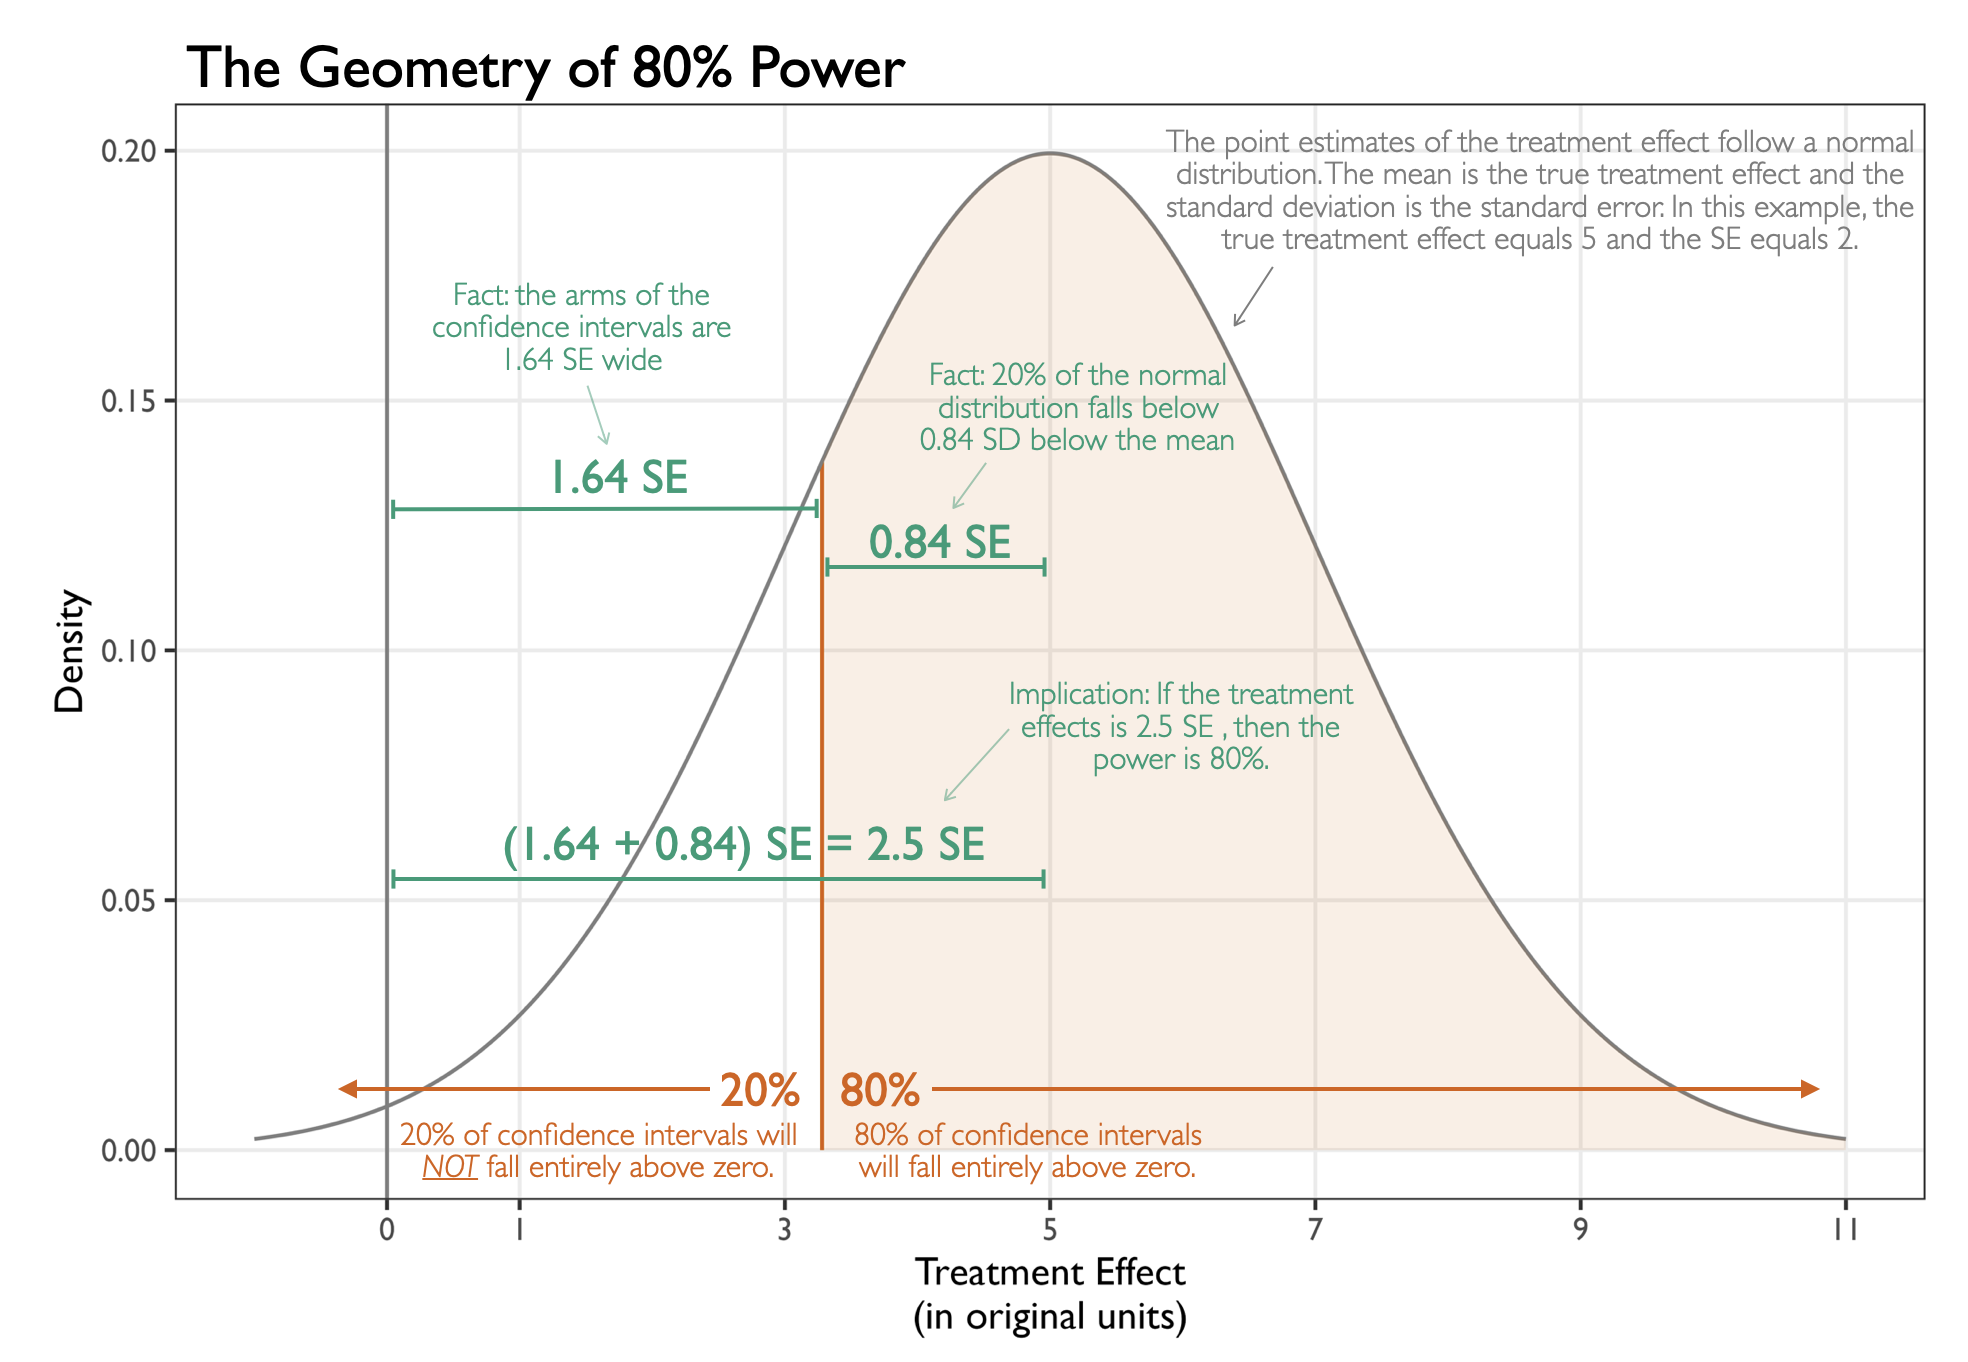
\includegraphics[width=\linewidth]{geometry.png}
    \caption{This figure shows why experiments have 80\% power to detect effects that are 2.5 standard errors. First, the arms of the 90\% confidence interval are 1.64 standard errors wide, so the power of the study is the percent of the sampling distribution that is larger than 1.64 standard errors. If we plug 0.80 into the inverse of the normal CDF, we obtain 0.84. To position 80\% of the sampling distribution above 1.64 standard errors, the sampling distribution must be centered (1.64 + 0.84) standard errors = 2.48 standard errors above zero, which we can safely treat as 2.5.}
    \label{fig:intuition}
\end{figure}

\section*{Example: Evaluating Power for Fixed Sample Size}

In many research contexts, we do not choose the sample size. 
For example, it is common to include survey experiments on modules of the Cooperative Election Study (CES), which include 1,000 respondents. 
Or we might have the opportunity to include an experiment on a survey designed for another purpose. 
Or we might want to conduct an experiment on the entire population of interest. 
In this context, we simply need to know whether our already-determined sample size provides sufficient statistical power. 
Rules \ref{rule:sd-to-se}, \ref{rule:adjustment}, and \ref{rule:se-to-mde} allow us to work in this context (as well as Rules \ref{rule:existing-to-se} and \ref{rule:pilot-to-se} below).

As an example, imagine we are planning to replicate of Ahler and Sood's (\citeyear{Ahler2018}) finding that correcting respondents' misperceptions of their out-party reduces affective polarization.
If we are planning to replicate the finding on a CES module, then we will have 1,000 respondents total or 500 respondents in the treatment and control conditions. 
Do 1,000 respondents provide sufficient statistical power?

The original experiment shows that correcting respondents' misperceptions of their out-party reduces affective polarization. 
In their experiment, the treatment has two steps. 
First, Ahler and Sood (1) ask Republicans to report their perceptions of the percent of Democrats with certain demographic attributes and (2) ask Democrats to report their perceptions of the percent of Republicans with certain demographic attributes. 
After asking respondents to report their perceptions of the out-party, Ahler and Sood provide respondents with the correct information. 
Compared to a control group that was neither asked their perceptions nor given the correct information, the treatment group evaluated supporters of the out-party more favorably on a 101-point feeling thermometer scale. 
They estimate a treatment effect of 6.4 points on the 101-point scale with a 95\% confidence interval of [3,
10]. 
\cite{Broockman2022} directly replicate
Ahler and Sood's result and estimate the treatment effect is 3.9 with a 90\% confidence interval of
[1.1, 6.6].\footnote{\cite{Broockman2022} report a
  slightly different analysis in the main text of their paper. Most
  notably, they use the difference between evaluations of the ``people
  who are'' the in-party and ``people who are'' the out-party. Using
  their replication data, we run an analysis that treats evaluations of
  ``people who are'' the out-party as the outcome (instead of the
  difference). This latter, alternative analysis is similar to Ahler and
  Sood's approach, so I focus on it here.} 
In both cases, the 90\% confidence interval includes only positive effects, so the authors reject the null hypothesis that the treatment effect is less than or equal to zero and conclude that the treatment has the hypothesized positive effect on the feeling thermometer toward supporters of the out-party.

How could we use features of a reference population along with Rules \ref{rule:sd-to-se}, \ref{rule:adjustment}, and \ref{rule:se-to-mde} to evaluate our study?\footnote{
  In planning a replication of Ahler and Sood's result, we would ideally translate the standard errors from the original study (as well as Broockman, Kalla, and Westwood's (\citeyear{Broockman2022}) replication) into a standard error and minimum detectable effect for our study---see Rule \ref{rule:existing-to-se} below. 
  But, for the sake of this example, suppose this valuable information is not available.
  Also, triangulating from several sources is helpful.} 
Our goal is to use Rule \ref{rule:sd-to-se} to predict the standard error, use Rule \ref{rule:adjustment} to account for any control variables we plan to use, and use Rule \ref{rule:se-to-mde} to find the minimum detectable effect with 80\% and 95\% power. 
If that minimum detectable effect is sufficiently small, then we will say that our study has adequate statistical power.

\subsection*{Without Control Variables: Rules \ref{rule:sd-to-se} and \ref{rule:se-to-mde}}

Using Rule \ref{rule:sd-to-se}, the standard error will be about $\frac{2 \cdot \ \widetilde{SD(Y)}}{\sqrt{2 \cdot n}}$. 
In this context, $n = 500$ because we have two experimental conditions and $N = 1,000$ in a CES module. 
However, we must plug a suitable value for $\widetilde{SD(Y)}$ into the equation. For this application, and many others, we can think of $\widetilde{SD(Y)}$ as the standard deviation of the outcome in the control group (or treatment group if that is easier).

In practice, we can look to standard deviations in reference populations ``like'' our experimental sample.\footnote{In a pinch, we can use the crude rule of thumb that the range of a variable tends to be about four times the standard deviation \citep{Wan2014}, so 101/4 = 25.25, though this rule should be used only as a first approximation, if used at all.} 
For example, the American National Elections Study (ANES) asks a \emph{similar} survey question. 
The ANES version asks respondents to report their feelings toward the Democratic [Republican] party, while Ahler and Sood ask respondents to report their feelings toward \emph{supporters of} the Democratic [Republican] party. 
The standard deviation of the responses to the similar ANES question is 20.8.

Using Rule \ref{rule:sd-to-se}, the standard error in our replication will be about $\frac{2 \cdot \widetilde{SD(Y)}}{\sqrt{2 \cdot n}} = \frac{2 \cdot 20.8}{\sqrt{2 \cdot 500}} = 1.32$.
Using Rule \ref{rule:se-to-mde}, a standard error of 1.32 means that we will have 80\% power to detect a treatment effect of $2.5 \cdot SE = 2.5 \cdot 1.32 = 3.30$ points on the 101-point scale and have 95\% power to detect a treatment effect of $3.3 \cdot SE = 3.3 \cdot 1.32 = 4.36$ points. 
As substantive experts, if we determine that these effects are acceptable (e.g., they correspond to the smallest substantively meaningful effect), then the experiment has adequate statistical power.


\subsection*{With Control Variables: Rules \ref{rule:sd-to-se}, \ref{rule:adjustment}, and \ref{rule:se-to-mde}}

To shrink the standard error (and the minimum detectable effect along with it), we can consider the adjustment strategy of \cite{Broockman2022}. 
They control for a seven-party party identification scale and partisan strength. 
Rule \ref{rule:adjustment} states that regression adjustment will shrink the unadjusted standard error by about $\left\lbrack 1 - \sqrt{ 1 - \widetilde{R^{2}} } \right\rbrack \cdot 100\%$, but we need to choose a suitable value of $\widetilde{R^{2}}$ to plug into the equation.

In the 2020 ANES, the seven-point party identification scale and partisan strength scale have $R^{2}$ of 5\% for the similar feeling thermometer toward the Democratic and Republican parties (rather than ``supporters of'' those parties). 
For $\widetilde{R^{2}} = 5\%,$ this adjustment strategy will shrink the standard error by about $\left\lbrack 1 - \sqrt{ 1 - \widetilde{R^{2}} } \right\rbrack = \left\lbrack 1 - \sqrt{1 - 0.05} \right\rbrack = 2.5\%$.
This strategy is perhaps worth pursuing, but will not change the standard error dramatically.\footnote{It seems reasonable, too, that these two variables will explain less variation in feelings toward ``supporters of'' the Democratic and Republican parties, so this $R^{2}$ of 5\% might be too high. Indeed, re-analysis of Broockman, Kalla, and Westwood's data shows that these two control variables produce an $R^{2}$ of 0.9\% in the control group and 1.8\% in the treatment group. An $R^{2}$ of 1.4\% (which is the average of the two) will shrink the standard error by about 0.7\%. This difference is negligible compared to a strategy without control variables.}

Adding the adjustment to our calculation, our standard error will be about $\frac{2 \cdot \widetilde{SD(Y)}\cdot \sqrt{1 - \widetilde{R^{2}}}}{\sqrt{2 \cdot n}} = \frac{2 \cdot 20.8 \cdot \sqrt{1 - 0.05}}{\sqrt{2 \cdot 500}} = 1.28$.
Using Rule \ref{rule:se-to-mde}, a standard error of 1.28 means that we will have 80\% power to detect a treatment effect of $2.5 \cdot SE = 2.5 \cdot 1.28 = 3.20$ points on the 101-point scale and have 95\% power to detect a treatment effect of $3.3 \cdot SE = 3.3 \cdot 1.28 = 4.22$ points. 
The minimum detectable effects using Broockman, Kalla, and Westwood's adjustment strategy are practically the same as those without any adjustment.

However, \cite{Clifford2021} offer a potentially promising approach here. 
They suggest measuring the outcome both before and after the treatment and then controlling for the pre-treatment measure. 
This pre-treatment measure should be \emph{strongly} related to the post-treatment outcome. 
If we let $\widetilde{R^{2}} = 40\%$---though we should do additional work to confirm this working assumption\footnote{
  In a small pilot study, \cite{Culter2024} validate a strategy of measuring the feelings toward supporters of the out-party before and after the treatment. 
  In their small pilot with 250 respondents, they find that the pre-treatment measure has an $R^{2}$ of about 73\%. 
  This suggests that the pre-post strategy will shrink the SE by about 48\%.}---then the standard error will be about $\frac{2 \cdot 20.8 \cdot \sqrt{1 - 0.40}}{\sqrt{2 \cdot 500}} = 1.02$. 
For a standard error of 1.02, we will have 80\% power to detect a treatment effect of $2.5 \cdot SE = 2.5 \cdot 1.02 = 2.55$ points on the 101-point scale and 95\% power to detect a treatment effect of $3.3 \cdot SE = 3.3 \cdot 1.02 = 3.37$ points. 
This adjustment strategy might make a difference in whether we consider our 1,000-respondent study adequately powered!

\section*{Rule \ref{rule:sd-to-sample-size}: From the SD to the Sample Size}

Rule \ref{rule:se-to-mde} is helpful---it gives us the minimum detectable effect for a given study.
But it does not produce the sample size that we need to obtain 80\% or 95\% power. 
To find the sample size that produces our desired minimum detectable effect (i.e., usually the smallest substantively meaningful effect), we can combine Rules \ref{rule:sd-to-se}, \ref{rule:adjustment}, and \ref{rule:se-to-mde}. 
Suppose we want our experiment to have 80\% power to detect the effect $\widetilde{\tau}$.
Then we need $\widetilde{\tau} = \frac{SE}{2.5} = \frac{\frac{\widetilde{SD(Y)}}{\sqrt{2 \cdot n}}}{2.5}$.
Solving for $n$, we find that we will need $2 \cdot \left( \frac{2.5 \cdot \widetilde{SD(Y)}}{\widetilde{\tau}} \right)^{2}$ respondents per condition to obtain 80\% power. 
If we are adjusting for control variables, we need $2 \cdot \left( \frac{\dot{2.5 \cdot \widetilde{SD(Y)} \cdot \sqrt{\left( 1 - \widetilde{R^{2}} \right)}}}{\widetilde{\tau}} \right)^{2}$ respondents per condition for 80\% power. For 95\% power to detect the effect $\widetilde{\tau}$, the factor changes from 2.5 to 3.3 and we need $2 \cdot \left( \frac{3.3 \cdot \widetilde{SD(Y)}}{\widetilde{\tau}} \right)^{2}$ or $2 \cdot \left( \frac{3.3 \cdot \dot{\widetilde{SD(Y)} \cdot \sqrt{\left( 1 - \widetilde{R^2} \right)}}}{\widetilde{\tau}} \right)^{2}$ respondents per condition, respectively.\footnote{This leads to another useful rule of thumb, though this one is rough. Suppose that we are interested in effects that are 10\% of a standard deviation. Then the term $\left( \frac{\widetilde{SD(Y)}}{\widetilde{\tau}} \right)^{2}$ equals 100, so we can simply multiply the factors $2 \cdot {2.5}^{2} = 12.5$ and $2 \cdot {3.3}^{2} = 21.8$ by 100 to find the required sample sizes of 1,250 and 2,180 per condition to detect these ``small'' effects with 80\% and 95\% power.}

\begin{restatable}[SD to Sample Size]{rule0}{rulesdtosamplesize}
\label{rule:sd-to-sample-size}
We can use features of a reference population to predict the sample size we will need in a planned study. 
For 80\% power to detect the treatment effect $\widetilde{\tau}$, the sample size per condition will need to be about $2 \cdot \left( \frac{2.5 \cdot \widetilde{SD(Y)}}{\widetilde{\tau}} \right)^{2}$ (or $2 \cdot \left( \frac{\dot{2.5 \cdot \widetilde{SD(Y)} \cdot \sqrt{\left( 1 - \widetilde{R^{2}} \right)}}}{\widetilde{\tau}} \right)^{2}\ $if including control variables), where $\widetilde{SD(Y)}$ is the standard deviation of the outcome in a reference population and $\widetilde{R^2}$ is the $R^2$ of a regression of the outcome on the control variables in a reference population.
For 95\% power, the factor changes from 2.5 to 3.3.
\end{restatable}
\section*{Rule \ref{rule:existing-to-se}: From an Existing Study to the Standard Error}

The square root law tells us that the standard error depends on the sample size by a factor of $\frac{1}{\sqrt{n}}$. 
For example, the classical standard errors that I use to motivate these rules have the form $SE_{\widehat{\tau}}^{classic} = \frac{2 \cdot \sigma}{\sqrt{2 \cdot n}} = \frac{2 \cdot \sigma}{\sqrt{2}} \cdot \frac{1}{\sqrt{n}}$.
This implies a useful relationship between two studies A and B that vary in their sample size.\footnote{Or less exactly, but more usefully, two \emph{similar} studies that vary in their sample size.} 
The ratio of two standard errors ${SE}_{\widehat{\tau}}^{A}$ and ${SE}_{\widehat{\tau}}^{B}$ with sample sizes $n^{A}$ and $n^{B}$ per condition, respectively, has the form $\frac{SE_{\widehat{\tau}}^{A}}{SE_{\widehat{\tau}}^{B}} = \frac{\frac{2 \cdot \sigma}{\sqrt{{2 \cdot n}^{A}}}}{\frac{2 \cdot \sigma}{\sqrt{{2 \cdot n}^{B}}}}$.
The two $\frac{2 \cdot \sigma}{\sqrt{2}}$ cancel and we have $\frac{SE_{\widehat{\tau}}^{A}}{SE_{\widehat{\tau}}^{B}} = \sqrt{\frac{n^{B}}{n^{A}}}$.
Solving for $SE_{\widehat{\tau}}^{B}$, we have $SE_{\widehat{\tau}}^{B} = \sqrt{\frac{n^{A}}{n^{B}}} \cdot SE_{\widehat{\tau}}^{A}$.
Thus, if we know the sample size and standard error of an existing study, then we can use the existing study to predict the standard error in our planned study: our standard error will be about $\sqrt{\frac{n^{existing}}{n^{planned}}} \cdot SE_{\widehat{\tau}}^{existing}$.

\begin{restatable}[Existing Study to SE]{rule0}{ruleexistingtose}
\label{rule:existing-to-se}
We can use an existing, similar study to predict the standard error of the estimated treatment effect in a planned study. The standard error will be about $\sqrt{\frac{n^{existing}}{n^{planned}}} \cdot SE_{\widehat{\tau}}^{existing}$, where $n^{existing}$ is the number of respondents per condition in the existing study, $SE_{\widehat{\tau}}^{existing}$ is the estimated standard error in the existing study, and $n^{planned}$ is the number of respondents per condition in the planned study. 
\end{restatable}

\section*{Rule \ref{rule:existing-to-sample-size}: From an Existing Study to the Sample Size}

We can also use an existing study to predict the sample size we need to obtain a desired power level.
From Rule \ref{rule:existing-to-se}, we know that $SE_{\widehat{\tau}}^{planned} = \sqrt{\frac{n^{existing}}{n^{planned}}} \cdot {\widehat{SE}}_{\widehat{\tau}}^{planned}$.
If we want 80\% power to detect the effect $\widetilde{\tau}$ in our planned study, then we need $SE_{\widehat{\tau}}^{planned} = \ \frac{\widetilde{\tau}}{2.5}$ (see
Rule \ref{rule:se-to-mde}). Plugging this into Rule \ref{rule:existing-to-se} and solving for $n^{planned}$, we will need about $n^{existing} \cdot \left( \frac{2.5}{\widetilde{\tau}} \cdot {\widehat{SE}}_{\widehat{\tau}}^{existing} \right)^{2}$ respondents per condition. 
For 95\% power, we will need about $n^{exisiting} \cdot \left( \frac{3.3}{\widetilde{\tau}} \cdot {\widehat{SE}}_{\widehat{\tau}}^{existing} \right)^{2}$ respondents per condition.

\begin{restatable}[Existing Study to Sample Size]{rule0}{ruleexistingtosamplesize}
\label{rule:existing-to-sample-size}
We can use an existing, similar study to predict the sample size we will need in a planned study. For 80\% power to detect the treatment effect $\widetilde{\tau}$, we will need about $n^{existing} \cdot \left\lbrack \frac{2.5}{\widetilde{\tau}} \cdot {\widehat{SE}}_{\widehat{\tau}}^{existing} \right\rbrack^{2}$ respondents per condition, where $n^{existing}$ is the number of respondents per condition in the existing study and $SE_{\widehat{\tau}}^{existing}$ is the estimated standard error in the existing study
For 95\% power, the factor changes from 2.5 to 3.3.
\end{restatable}

\section*{Rule \ref{rule:pilot-to-se}: From Pilot Data to the SE}

It is common to run a small pilot study prior to the experiment for reasons unrelated to statistical power.\footnote{
  Importantly, one should \textit{not} use pilot data to estimate the treatment effect $\widehat{\tau}$. 
  Any pilot study will not be sufficiently precise to provide a useful estimate of the treatment effect.
  }
For example, we might like to learn whether respondents can accurately remember certain details of a vignette. 
If we have pilot data available, we can also use these pilot data to predict statistical power. 
Suppose, for example, that we have tentatively planned to run a full study with 1,000 respondents. 
We might run a pilot study on 100 respondents to make sure that no issues arise. 
We can perform the planned analysis on the pilot data and use Rule \ref{rule:existing-to-se} to predict the standard errors (and minimum detectable
effect) in the full study.\footnote{We should not pay attention to the
point estimates in the pilot data; the point estimates are too noisy to
be useful for any purpose.} 
For example, if the small pilot has a standard error of 2.0, then a good guess of the standard error in the full study is $\sqrt{\frac{100}{1,000}} \cdot 2.0 = 0.32 \cdot 2.0 = 0.63$.

However, translating the standard error from a small pilot study is meaningfully different from translating the standard error from another full study. Recall that the standard error estimate from the pilot data is only an \emph{estimate.} 
And while the standard error estimate is usually accurate, pilot studies are typically small enough to worry about substantially under-estimating the standard error (and thus
over-estimating power). 
To protect against running an under-powered study, I recommend predicting the standard error \emph{conservatively} from pilot data. 

To understand how severely you might under-estimate (or over-estimate)
the standard error using Rule \ref{rule:existing-to-se}, recall the that standard error of a sample standard deviation is about $SE\left( \text{sample SD} \right) = \ \text{sample SD} \cdot \sqrt{\frac{1}{4 \cdot n}}$ so that the factor $\sqrt{\frac{1}{4 \cdot n}} \cdot 100\%$ gives us a typical error in the estimate of the standard error as a percentage. 
For $N = 100$, the standard error estimate is typically off by about 7\% (either too high or too low), with errors larger than about 14\% being unusual. 
To protect against an under-powered study, we can increase the predicted standard error by a factor of $2 \cdot \sqrt{\frac{1}{4 \cdot n}} + 1 = \ \sqrt{\frac{1}{n}} + 1$, which roughly corresponds to the upper bound of a 95\% confidence interval for the standard error. 
Plugging this conservative standard error into Rule \ref{rule:existing-to-se} above, we obtain $\sqrt{\frac{n^{pilot}}{n^{planned}}}\ \left\lbrack \left( \sqrt{\frac{1}{n^{pilot}}} + 1 \right) \cdot {\widehat{SE}}_{\widehat{\tau}}^{pilot} \right\rbrack$
as a \emph{conservative} estimate of the standard error. 

\begin{restatable}[Pilot Data to SE]{rule0}{rulepilottose}
\label{rule:pilot-to-se}
We can use pilot data to predict the standard error of the estimated treatment effect in a planned study. Conservatively, the standard error will be about $\sqrt{\frac{n^{pilot}}{n^{planned}}}\ \left\lbrack \left( \sqrt{\frac{1}{n^{pilot}}} + 1 \right) \cdot {\widehat{SE}}_{\widehat{\tau}}^{pilot} \right\rbrack$, where $n^{pilot}$ is the number of respondents per condition in the pilot data, $SE_{\widehat{\tau}}^{pilot}$ is the estimated standard error using the pilot data, and $n^{planned}$ is the number of respondents per condition in the planned study. 
\end{restatable}

\section*{Rule \ref{rule:pilot-to-sample-size}: From Pilot Data to the Sample Size}

Perhaps most importantly, we can use the logic of Rule \ref{rule:existing-to-sample-size} to make adjustments to the sample size of the planned study. 
Suppose that we want to design an experiment with 80\% power to detect the effect $\widetilde{\tau}$. 
By Rule \ref{rule:se-to-mde}, we need the standard error to be $\frac{\widetilde{\tau}}{2.5}$. 
Using Rule \ref{rule:pilot-to-se}, we can conservatively predict that the standard error will be $\sqrt{\frac{n^{pilot}}{n^{planned}}}\ \left\lbrack \left( \sqrt{\frac{1}{n^{pilot}}} + 1 \right) \cdot {\widehat{SE}}_{\widehat{\tau}}^{pilot} \right\rbrack$.
Setting this equal to $\frac{\widetilde{\tau}}{2.5}$ and solving for $n^{planned}$, we can conservatively predict that $n^{pilot} \cdot \left\lbrack \frac{2.5}{\widetilde{\tau}} \cdot \left( \sqrt{\frac{1}{n^{pilot}}} + 1 \right) \cdot {\widehat{SE}}_{\widehat{\tau}}^{pilot} \right\rbrack^{2}$ respondents per condition will give us 80\% power to detect the effect $\widetilde{\tau}$.

\begin{restatable}[Pilot Data to Sample Size]{rule0}{rulepilottosamplesize}
\label{rule:pilot-to-sample-size}
We can use pilot data to conservatively predict the sample size we will need in a planned study. 
For 80\% power to detect the treatment effect $\widetilde{\tau}$, we will (conservatively) need about $n^{pilot} \cdot \left\lbrack \frac{2.5}{\widetilde{\tau}} \cdot \left( \sqrt{\frac{1}{n^{pilot}}} + 1 \right) \cdot {\widehat{SE}}_{\widehat{\tau}}^{pilot} \right\rbrack^{2}$ respondents per condition, where $n^{pilot}$ is the number of respondents per condition in the pilot data and $SE_{\widehat{\tau}}^{pilot}$ is the estimated standard error using the pilot data
For 95\% power, the factor changes from 2.5 to 3.3.
\end{restatable}

\section*{More Examples: Finding the Sample Size}

In the examples above, we imagined a research context in which the sample size was not under our control. 
But any many contexts, we can control (or must choose) the sample size. 
Continuing our example of Ahler and Sood's (\citeyear{Ahler2018}) experiment from above, we can use features of a reference population, similar existing studies, and pilot data to predict the required sample size. 
For the Ahler and Sood example, we have all three available. 
For simplicity, suppose that we would like 95\% power to detect a treatment effect of 3 points on the 101-point scale.\footnote{A 3-point effect on the 101-point scale is the lower bound of Ahler and Sood's 95\% confidence interval.}

\subsection*{Features of a Reference Population}

Above, we use the ANES to motivate setting $\widetilde{SD(Y)}$ to 20.8 and $\widetilde{R^{2}}$ to 5\%. 
Rule \ref{rule:sd-to-sample-size} tells us that, without control variables, we will need about $2 \cdot \left( \frac{3.3 \cdot \widetilde{SD(Y)}}{\widetilde{\tau}} \right)^{2} = 2 \cdot \left( \frac{3.3 \cdot 20.8}{3} \right)^{2} = 1,050$ respondents per condition for 95\% power. 
With control variables, this becomes ${2 \cdot \left( \frac{\widetilde{3.3 \cdot SD(Y)} \cdot \sqrt{\left( 1 - \widetilde{R^{2}} \right)}}{\widetilde{\tau}} \right)}^{2} = 2 \cdot \left( \frac{3.3 \cdot 20.8 \cdot \sqrt{(1 - 0.05)}}{3} \right)^{2} = 995$.

\subsection*{An Existing Study: \cite{Ahler2018}}

\cite{Ahler2018} have about 268 respondents per condition with a
standard error of about 1.8 on the 101-point scale. 
If we mimic their design, then we can use Rule \ref{rule:existing-to-sample-size} to predict that we will need $n^{existing} \cdot \left\lbrack \frac{3.3}{\widetilde{\tau}} \cdot {\widehat{SE}}_{\widehat{\tau}}^{existing} \right\rbrack^{2} = 268 \cdot \left\lbrack \frac{3.3}{3} \cdot 1.8 \right\rbrack^{2} = 1,051$ respondents per condition for 95\% power to detect a treatment effect of 3 points on the 101-point scale.

\subsection*{An Existing Study: \cite{Broockman2022}}

\cite{Broockman2022} have about 502 respondents per condition with a standard error of about 1.67 on the 101-point scale.
If we mimic their design, then we can use Rule \ref{rule:existing-to-sample-size} to predict that we will need $n^{existing} \cdot \left\lbrack \frac{3.3}{\widetilde{\tau}} \cdot {\widehat{SE}}_{\widehat{\tau}}^{existing} \right\rbrack^{2} = 502 \cdot \left\lbrack \frac{3.3}{3} \cdot 1.7 \right\rbrack^{2} =1,694$ respondents per condition for 95\% power to detect a treatment effect of 3 points on the 101-point scale.\footnote{
  In Broockman, Kalla, and Westwood's data, the standard deviation of the outcome is about 27, which is much larger than the standard deviation of the similar measure in the ANES (about 21) and the standard deviation of Ahler and Sood's measure (about 22). 
  This highlights the importance of triangulating power calculations using multiple sources to motivate the assumptions.
  }

\subsection*{A Pilot Study: \cite{Culter2024}}

\cite{Culter2024} conduct a pilot study with about 85 respondents per condition. 
Their study uses the pre-post strategy suggested by \cite{Clifford2021} and they include the pre-treatment measure as a control variable. 
They analyze the small pilot data set as they plan to analyze the full data set and find a standard error of 2.13. 
Using Rule \ref{rule:pilot-to-sample-size}, they will need (conservatively) about
$n^{pilot} \cdot \left\lbrack \frac{3.3}{\widetilde{\tau}} \cdot \left( \sqrt{\frac{1}{n^{pilot}}} + 1 \right) \cdot {\widehat{SE}}_{\widehat{\tau}}^{pilot} \right\rbrack^{2} = 85 \cdot \left\lbrack \frac{3.3}{3} \cdot \left( \sqrt{\frac{1}{85}} + 1 \right) \cdot 2.13 \right\rbrack^{2} = 573$ respondents per condition for 95\% power to detect a treatment effect of 3 points on the 101-point scale. Cutler, Pietryka, and Rainey's approach requires many fewer observation because their pre-treatment measure is highly predictive of the outcome.

\section*{Rule \ref{rule:80-to-95}: From 80\% Power to 95\% Power}

In thinking about the tradeoff between 80\% and 95\% power it can be helpful to have a rule connecting sample size requirements. 
Recall from
Rule \ref{rule:existing-to-se} that $\frac{SE_{\widehat{\tau}}^{A}}{SE_{\widehat{\tau}}^{B}} = \ \sqrt{\frac{n^{B}}{n^{A}}}$.
For an assumed treatment effect $\widetilde{\tau}$, the standard errors that yield 80\% and 95\% power are given by $\frac{\widetilde{\tau}}{2.5}$
and $\frac{\widetilde{\tau}}{3.3}$, respectively. 
Then we have $\frac{SE_{\widehat{\tau}}^{A}}{SE_{\widehat{\tau}}^{B}} = \frac{\frac{\widetilde{\tau}}{2.5}}{\frac{\widetilde{\tau}}{3.3}} = \frac{3.3}{2.5} = \sqrt{\frac{n^{B}}{n^{A}}}$.
Then we can see that $\frac{n^{B}}{n^{A}}$ = $\left( \frac{3.3}{2.5} \right)^{2}$ = 1.74. This means that to increase the power from 80\% to 95\%, we need increase our sample size by about 74\%. 
With less rounding error, this becomes 75\%.

\begin{restatable}[80\% to 95\% Power]{rule0}{ruleconvert}
\label{rule:80-to-95}
Increasing the sample size by 75\% will increase the power from 80\% to about 95\%.
\end{restatable}

\section*{How Are Interactions Different?}

Up to this point in the paper, I have focused on a hypothesis about the treatment effect (i.e., ``average treatment effect'' or ATE). 
But what if we have a hypothesis about an \emph{interaction} (i.e., a difference in treatment effects across two scenarios)? 
The general logic of the rules extends to the interaction, with two minor modifications.

Assume a $2 \times 2$ factorial design with two treatments. 
Then we have potential outcomes $\mathcal{Y}_{i}(1, 1)$ if assigned to both treatments, $\mathcal{Y}_{i}(1,0)$ if assigned to the first treatment, $\mathcal{Y}_{i}(0,1)$ if assigned to the second treatment, and $\mathcal{Y}_{i}(0,0)$ if assigned neither treatment for respondent $i$ of $N$. 
Then we can define the interaction as $\delta = \left\lbrack \ \frac{1}{N}\sum_{i = 1}^{N}{\mathcal{Y}_{i}(1,\ 1)\ } - \frac{1}{N}\sum_{i = 1}^{N}{\mathcal{Y}_{i}(0,\ 1)} \right\rbrack - \left\lbrack \ \frac{1}{N}\sum_{i = 1}^{N}{\mathcal{Y}_{i}(1,\ 0)\ }- \frac{1}{N}\sum_{i = 1}^{N}{\mathcal{Y}_{i}(0,\ 0)} \right\rbrack$.

Imagine we assign $n$ respondents to each of the four conditions. 
We create two indicator variables $D_{1}$ and $D_{2}$ that equal 1 if the respondent is assigned to the first and second treatment, respectively, and 0 otherwise. 
Then we create the observed outcome $Y = \mathcal{Y}\left( D_{1},\ D_{2} \right)$. 
Then we estimate the interaction in practice using least squares estimates of the model
$Y = \beta_{0} + {\beta_{1} \cdot D}_{1}{{+ \ \beta}_{2} \cdot D}_{2} + \delta \cdot D_{1} \cdot D_{2} + \epsilon$.
The parameter $\delta$ is the interaction. 
Inference about this parameter is the same as described above (least squares regression and robust standard errors; inferences about $\delta$ using the 90\% confidence interval). 
By assuming $\epsilon_{i} \sim N\left( 0,\ \sigma^{2} \right)$, the classical variance for the least squares estimates of the parameter vector $\mathbf{\beta} = \ \lbrack\beta_{0},\ \beta_{1},\ \beta_{2},\ \delta\rbrack'$ is $Var\left( \widehat{\mathbf{\beta}} \right) = \left( \mathbf{X}^{'}\mathbf{X} \right)^{- 1}\sigma^{2}$ for the design matrix $\mathbf{X} = \lbrack 1,\ D_{1},\ D_{2},\ D_{1} \cdot D_{2}\rbrack$. 
The experimental design requires $n$ repetitions of each of the four unique rows of $\mathbf{X}$, which allows us to simplify $\left( \mathbf{X}^{'}\mathbf{X} \right)^{- 1}$ and find that the bottom right element of $\left( \mathbf{X}^{'}\mathbf{X} \right)^{- 1}\sigma^{2}$---the variance of $\widehat{\delta}$---equals $\frac{4}{n}$. 
This gives us $SE_{\widehat{\delta}}^{classic} = \ \sqrt{\frac{{4 \cdot \sigma}^{2}}{n}} = \frac{2 \cdot \sigma}{\sqrt{n}}$, where $n$ represents the number of respondents assigned to each condition.\footnote{Alternatively, we can think of the estimate of the
  interaction effect as the difference in differences of sample means
  $\widehat{\delta} = \left\lbrack \ {\overline{Y}}_{11}-\ {\overline{Y}}_{01} \right\rbrack - \left\lbrack \ {\overline{Y}}_{10}-\ {\overline{Y}}_{00} \right\rbrack$,
  where ${\overline{Y}}_{11}$ represents the sample average for respondents
  where $D_{1} = 1$ and $D_{2} = 1$ and so on. Assuming
  independence of the sample means, the variance of these differences is
  the sum of the variances of each term, so that
  $Var(\widehat{\delta}$) =
  $\frac{\sigma^{2}}{n} + \ \frac{\sigma^{2}}{n} + \frac{\sigma^{2}}{n} + \frac{\sigma^{2}}{n} = \frac{4{\cdot \sigma}^{2}}{n}$.
  This also give us
  $SE_{\widehat{\delta}}^{classic} = \ \sqrt{\frac{{4 \cdot \sigma}^{2}}{n}} = \frac{2 \cdot \sigma}{\sqrt{n}}$.
  This motivation that Gelman uses in his widely-shared blog post
  (accessed May 3, 2024; persistent link:
  \url{https://archive.md/FOTo7}).} 

Two of the rules above change for interactions.

\begin{itemize}
\item 
  \textbf{A Modification to Rules \ref{rule:sd-to-se} and \ref{rule:sd-to-sample-size}.} 
  Rules \ref{rule:sd-to-se} and \ref{rule:sd-to-sample-size} help us use features of a reference population to predict the standard error for the estimate of a treatment effect and approximate the required sample size, respectively. 
  When estimating an interaction rather than a treatment effect, we need to adjust these approximations. 
  \begin{itemize}
      \item   First, Rule \ref{rule:sd-to-se} requires adjustment. As explained above, the standard error for the estimated interaction is about $\frac{2 \cdot \widetilde{SD(Y)}}{\sqrt{n}}$ rather than $\frac{2 \cdot \widetilde{SD(Y)}}{\sqrt{2 \cdot n}}$ for the treatment effect.
      \item Second, Rule \ref{rule:sd-to-sample-size} requires adjustment. 
      Suppose we want our experiment to have 80\% power to detect the interaction $\widetilde{\delta}$. 
      Then we need $\widetilde{\delta} = 2.5 \cdot SE = 2.5 \cdot \frac{2 \cdot \widetilde{SD(Y)}}{\sqrt{n}}$. 
      Solving for $n$, we find that $n = 4 \cdot \left( \frac{2.5 \cdot \widetilde{SD(Y)}}{\widetilde{\delta}} \right)^{2}$. 
      If we are adjusting for control variables, we have $4 \cdot \left( \frac{\dot{2.5 \cdot \widetilde{SD(Y)} \cdot \sqrt{\left( 1 - \widetilde{R^{2}} \right)}}}{\widetilde{\delta}} \right)^{2}$. 
      Notice that the first factor changes from 2 in Rule \ref{rule:sd-to-se} to 4 for interaction. 
      For 95\% power, the factor changes from 2.5 to 3.3.
  \end{itemize}
\item \textbf{A Modification to Rules \ref{rule:pilot-to-se} and \ref{rule:pilot-to-sample-size}.} Second, Rules \ref{rule:pilot-to-se} and \ref{rule:pilot-to-sample-size} require a small adjustment to account for the change from $N = 2 \cdot n$ in the treatment effect context to $N = 4 \cdot n$ in the interaction context---the SE will be more accurate with a larger total sample size. 
The adjustment factor changes from $\left( \sqrt{\frac{1}{n^{pilot}}} + 1 \right)$ in the treatment effect context to $\overset{\text{modified}}{\overbrace{\sqrt{\frac{1}{2 \cdot n^{pilot}}}}} + 1$ in the interaction context.
\end{itemize}

Comparing the standard error for the interaction to the standard error for the treatment effect leads to three important observations. First, for the treatment effect, we had $SE_{\widehat{\tau}}^{classic} = \ \sqrt{\frac{\sigma^{2}}{2 \cdot n \cdot \frac{1}{4}}} = \frac{2 \cdot \sigma}{\sqrt{2 \cdot n}} = \ \frac{1}{\sqrt{2}} \cdot \frac{2 \cdot \sigma}{\sqrt{n}}$; thus the standard error for the interaction is $\sqrt{2}$ times larger (about 41\% larger) than the standard error for the treatment effect. In order to make the standard errors the same, we need to double the sample size \textit{in each condition}.
Second, the $2 \times 2$ factorial design has twice as many conditions and thus requires twice the sample size in total. 
Third, the interaction is likely much smaller than the treatment effect. 
In a widely shared blog post, Andrew Gelman famously suggests that ``you
need 16 times the sample size to estimate an interaction than to
estimate a main effect'' (accessed May 3, 2024; persistent link:
\url{https://archive.md/FOTo7}). 
While this rule is too crude to apply generally---it makes strong assumptions about the treatment effect of interest---it does starkly highlight the demands of estimating an interaction relative to the treatment effect. 
It can help our intuition to partition the Gelman's 16x claim into its constituent parts: you need twice the number of respondents per condition for a similarly precise estimate, twice the number of conditions, and four times the number of respondents when the parameter is half the size.

\section*{Example: Interactions}

\cite{Robbins2024} study how respondents evaluate in-party legislators when they criticize an out-party president following a covert operation. 
They hypothesize that Republicans, for example, will report higher approval of Republican legislators that are more critical of the Democratic president, but that this effect will be much larger when the operation fails than when the operation succeeds. 
To test their hypothesis, they design a $2 \times 2$ factorial experiment. 
In each condition, a vignette describes (1) a covert operation that succeeds or fails and (2) legislators that aggressively criticize or ignore the operation.

Informed by \cite{Myrick2020}, the authors expected that criticism would increase approval by about 0.33 points on a seven-point scale when the operation succeeded, but by about 1.00 points when the operation failed.
This implies an interaction of about 0.67 points.

\cite{Myrick2020} conducted a similar experiment and measured her outcomes similarly. After analyzing her data closely, the authors expected their seven-point approval outcome would have a standard deviation of about 2.0. 
Using Rule \ref{rule:sd-to-se} (and modifying for interaction), the authors would need about $4 \cdot \left( \frac{2.5 \cdot 2.0}{0.67} \right)^{2} = 223$ respondents per condition (or 892 respondents in total) for 80\% power to detect an interaction of 0.67. 
For 95\% power, the authors would need about $4 \cdot \left( \frac{3.3 \cdot 2.0}{0.67} \right)^{2} = 389$ respondents per condition (or 1,556 respondents in total).

The authors also completed a pilot study with 75 respondents per condition. 
They conducted their planned analysis on the pilot data and estimated a standard error of 0.40 for the interaction. 
Using Rule \ref{rule:pilot-to-sample-size}, conservatively, the authors would need about $n^{pilot} \cdot \left\lbrack \frac{2.5}{\widetilde{\tau}} \cdot \left( \sqrt{\frac{1}{{2 \cdot n}^{pilot}}} + 1 \right) \cdot {\widehat{SE}}_{\widehat{\tau}}^{pilot} \right\rbrack^{2} = 75 \cdot \left\lbrack \frac{2.5}{0.67} \cdot \left( \sqrt{\frac{1}{2 \cdot 75}} + 1 \right) \cdot 0.40 \right\rbrack^{2} = 195$ respondents per condition (or 780 respondents total) to have 80\% power to detect an interaction of 0.67. 
For 95\% power, they would need about $75 \cdot \left\lbrack \frac{3.3}{0.67} \cdot \left( \sqrt{\frac{1}{2 \cdot 75}} + 1 \right) \cdot 0.40 \right\rbrack^{2} = 340$ respondents per condition (or 1,360 respondents total) to have 95\% power.\footnote{
  Robbins et al. ultimately used 375 respondents per condition (or 1,500 respondents total). 
  Using Rule \ref{rule:pilot-to-se}, the authors would conservatively predict the standard error would be about $\sqrt{\frac{n^{pilot}}{n^{planned}}}\  \cdot {\widehat{SE}}_{\widehat{\delta}}^{pilot} = \ \sqrt{\frac{75}{375}} \cdot 0.40 = 0.19$.
  In the full, 1,500-respondent study, the standard error was 0.18, which suggests a statistical power of about $1 - \ \Phi_{std}\left( 1.64 - \frac{\widetilde{\tau}}{SE} \right) = \ 1 - \Phi_{std}\left( 1.64 - \frac{0.67}{0.18} \right) = \ 98\%$ to detect an interaction of 0.67.
  }

\section*{How to Use the Rules}

Table \ref{tbl:how} shows how you can use the rules to establish that your planned experiment is well-powered. Broadly, there are three strategies, or ways to arrange our thinking:

\begin{enumerate}
\item For a given sample size and statistical power, show that the minimum detectable effect corresponds to a ``small'' effect, either the smallest substantively meaningful effect or the smallest plausible effect given the available evidence.
\item For given sample size and effect of interest, show that the statistical power of the experiment is greater than a chosen threshold (e.g., 80\% or 95\%).
\item For a given statistical power and effect of interest, show that the sample size meets (or exceeds) the required sample size.
\end{enumerate}

\noindent However, we should not draw strong distinctions between these strategies---the strategies differ only in the order in which the sample size, effect of interest, and statistical power are chosen. 
In the end, it simply matters that the three components combine to form a well-powered experiment.

To make each of these arguments, we can gather data from a variety of sources.

\begin{enumerate}
\item \textit{Features of a reference population.} We can find studies that measure our outcome (and perhaps control variables) on a similar population. We can use the standard deviation and $R^2$ in this reference population to predict the standard deviation and $R^2$ in our planned study. 
\item \textit{Existing similar study.} We can find an existing similar study. We can adjust the standard error estimates in the existing study to predict the standard error in our planned study. It is important that this study mimic the outcome and design of our planned study, though treatment (and treatment effect) can be quite different.
\item \textit{Pilot data.} We can use pilot data. We can adjust the standard error estimates from the pilot data to predict the standard error in our planned study. Because the standard error estimates in the pilot data will be quite noisy, we can make a conservative adjustment.
\end{enumerate}

\noindent Table \ref{tbl:how} describes how we might use these various strategies.

\begin{landscape}
\begin{table}[ht]
\centering
\caption{This table shows how we can use the rules to answer questions about the experiment using features of a reference population, existing studies, and pilot data.}\label{tbl:how}
\footnotesize % Making the font smaller
\setlength{\extrarowheight}{4pt} % Adding a little extra vertical padding to cells
\begin{tabularx}{\linewidth}{|>{\centering\arraybackslash}X|>{\centering\arraybackslash}m{3cm}|>{\centering\arraybackslash}m{3cm}|>{\centering\arraybackslash}m{5cm}|>{\centering\arraybackslash}X|} % Using fixed widths for some columns and X for the rest
\hline
\textbf{Goal} & \textbf{Source} & \textbf{Estimation Strategy} & \textbf{Required Information} & \textbf{Rule Sequence} \\
\hline
\multirow{4}{=}{I know my sample size and the statistical power I want. What is my minimum detectable effect?} & \multirow{2}{=}{\centering features of reference population} & no control variables & $SD(Y)$ in reference population & Rule \ref{rule:sd-to-se} $\rightarrow$ Rule \ref{rule:se-to-mde} \\
\cline{3-5}
 &  & control variables & $SD(Y)$ and $R^2$ of control variables in reference population & Rule \ref{rule:sd-to-se} $\rightarrow$ Rule \ref{rule:adjustment} $\rightarrow$ Rule \ref{rule:se-to-mde} \\
 \cline{2-5}
 & existing similar study & — & estimated standard error from existing study & Rule \ref{rule:existing-to-se} $\rightarrow$ Rule \ref{rule:se-to-mde} \\
 \cline{2-5}
 & pilot data & — & estimated standard error from pilot data & Rule \ref{rule:pilot-to-se} $\rightarrow$ Rule \ref{rule:se-to-mde} \\
\cline{1-5}

\hline
\multirow{4}{=}{I know my sample size and the effect of interest. What is my statistical power?} & \multirow{2}{=}{\centering features of reference population} & no control variables & $SD(Y)$ in reference population & Rule \ref{rule:sd-to-se} $\rightarrow$ Rule \ref{rule:power-z} \\
\cline{3-5}
 &  & control variables & $SD(Y)$ and $R^2$ of control variables in reference population & Rule \ref{rule:sd-to-se} $\rightarrow$ Rule \ref{rule:adjustment} $\rightarrow$ Rule \ref{rule:power-z} \\
 \cline{2-5}
 & existing similar study & — & estimated standard error from existing study & Rule \ref{rule:existing-to-se} $\rightarrow$ Rule \ref{rule:power-z} \\
 \cline{2-5}
 & pilot data & — & estimated standard error from pilot data & Rule \ref{rule:pilot-to-se} $\rightarrow$ Rule \ref{rule:power-z} \\
\cline{1-5}

\multirow{4}{=}{I know the statistical power I want and the effect of interest. What sample size do I need?} & \multirow{2}{=}{\centering features of reference population} & no control variables & $SD(Y)$ in reference population & Rule \ref{rule:sd-to-sample-size} \\
\cline{3-5}
 &  & control variables & $SD(Y)$ and $R^2$ of control variables in reference population & Rule \ref{rule:sd-to-sample-size} \\
 \cline{2-5}
 & existing similar study & — & estimated standard error from existing study & Rule \ref{rule:existing-to-sample-size} \\
 \cline{2-5}
 & pilot data & — & estimated standard error from pilot data & Rule \ref{rule:pilot-to-sample-size} \\
\hline
\end{tabularx}
\end{table}
\end{landscape}

\section*{Extensions}

\subsection*{What if I want power other than 80\% or 95\%?}

Throughout the paper, I discuss rules to obtain the minimum detectable effect and required sample size for 80\% or 95\% power. 
The rules for 80\% power have a factor of 2.5 that can be changed to 3.3 for 95\% power.
These factors are the minimum detectable effects, in standard errors (i.e., see Rule \ref{rule:se-to-mde}). 
What about other power levels? 
Table \ref{tbl:mdes} provides the minimum detectable effect, in standard errors, for a variety of power levels.\footnote{I round these minimum detectable effects to two significant digits. For greater precision, we can use \texttt{pnorm(0.95) + pnorm(0.80)}, where \texttt{0.80} corresponds to 80\% power and can be changed to the desired power level.} 
We can use these factors rather 2.5 for 80\% power (or 3.3 for 95\% power) in the relevant rules.
Table \ref{tbl:mdes} also provides the percent change in sample size to change the power from 80\% to various other levels (i.e., see Rule \ref{rule:80-to-95}).

\begin{table}[h]
\centering 
\caption{This table shows the minimum detectable effect, in standard errors, for a variety of power levels. We can use these values to find the minimum detectable effect for power levels other than 80\% and 95\% (i.e., as in Rule \ref{rule:se-to-mde}). We can also use these factors rather 2.5 for 80\% power (or 3.3 for 95\% power) in the relevant rules. For convenience, this table also shows the percent change in sample size required to change the statistical power from 80\% to the various levels.}\label{tbl:mdes}
\footnotesize % Making the font smaller
\renewcommand{\tabularxcolumn}[1]{>{\centering\arraybackslash}m{#1}} % Centering and middle aligning text in X columns
\setlength{\extrarowheight}{4pt} % Adding a little extra vertical padding to cells
\begin{tabularx}{\linewidth}{|X|X|X|} % Using tabularx to make the table fit the page width
\hline
\textbf{Power} & \textbf{Minimum Detectable Effect (in Standard Errors)} & \textbf{Percent Change in Sample Size from 80\% Power} \\
\hline
%10\%   & 0.4 & -98\% \\
%\hline
20\%   & 0.8 & -90\% \\
\hline
%30\%   & 1.1 & -80\% \\
%\hline
40\%   & 1.4 & -69\% \\
\hline
%50\%   & 1.6 & -56\% \\
%\hline
60\%   & 1.9 & -42\% \\
\hline
%70\%   & 2.2 & -24\% \\
%\hline
\textbf{80\%}   & \textbf{2.5} & \textbf{0\%} \\
\hline
90\%   & 2.9 & 39\% \\
\hline
\textbf{95\%}   & \textbf{3.3} & \textbf{75\%} \\
\hline
98\%   & 3.7 & 121\% \\
\hline
99\%   & 4.0 & 155\% \\
\hline
99.9\%  & 4.7 & 263\% \\
\hline
\end{tabularx}
\end{table}

\subsection*{What if I want to use a 95\% confidence interval?}

Checking that a 90\% confidence interval contains only values consistent with the research hypothesis corresponds to a size-0.05 test. 
However, some researchers prefer to use a 95\% confidence interval, which corresponds to size-0.025 test for directional claims. 
Table \ref{tbl:mdes2} provides the minimum detectable effects for researchers using a 95\% confidence interval.\footnote{
  I round these minimum detectable effects to two significant digits. 
  For greater precision, we could use \texttt{pnorm(0.975) + pnorm(0.80)}, where \texttt{0.80} corresponds to 80\% power and can be changed to the desired power level.
  } 
We can use these factors rather 2.5 for 80\% power in the relevant rules. 

\begin{table}[h]
\centering
\caption{This table is an alternate version of Table \ref{tbl:mdes} for researchers who wish to use a 95\% confidence interval rather than a 90\% confidence interval. The table shows the minimum detectable effect, in standard errors, for a variety of power levels. Researchers can use these values to find the minimum detectable effect for power levels other than 80\% and 95\% (i.e., as in Rule \ref{rule:se-to-mde}. Researchers can also use these factors rather 2.5 for 80\% power (or 3.3 for 95\% power) in the relevant rules. For convenience, this table also shows the percent change in sample size required to change the statistical power from 80\% to the various levels.}\label{tbl:mdes2}
\footnotesize % Making the font smaller
\renewcommand{\tabularxcolumn}[1]{>{\centering\arraybackslash}m{#1}} % Centering and middle aligning text in X columns
\setlength{\extrarowheight}{4pt} % Adding a little extra vertical padding to cells
\begin{tabularx}{\linewidth}{|X|X|X|} % Using tabularx to make the table fit the page width
\hline
\textbf{Power} & \textbf{Minimum Detectable Effect (in Standard Errors)} & \textbf{Percent Change in Sample Size from 80\% Power} \\
\hline
%10\%   & 0.7 & -94\% \\
%\hline
20\%   & 1.1 & -84\% \\
\hline
%30\%   & 1.4 & -74\% \\
%\hline
40\%   & 1.7 & -63\% \\
\hline
%50\%   & 2.0 & -51\% \\
%\hline
60\%   & 2.2 & -38\% \\
\hline
%70\%   & 2.5 & -21\% \\
%\hline
80\%   & 2.8 & 0\% \\
\hline
90\%   & 3.2 & 34\% \\
\hline
95\%   & 3.6 & 66\% \\
\hline
98\%   & 4.0 & 105\% \\
\hline
99\%   & 4.3 & 134\% \\
\hline
99.9\%  & 5.0 & 225\% \\
\hline
\end{tabularx}
\end{table}

For example, I noted above that \cite{Ahler2018} have about 268 respondents per condition with a standard error of about 1.8 on the 101-point scale. 
Suppose researchers want 80\% power to detect a treatment effect of 3 points on the 101-point scale with a 95\% confidence interval.
Using Rule \ref{rule:existing-to-sample-size} modified for a 95\% confidence interval, researchers would need about $n^{existing} \cdot \left\lbrack \frac{2.8}{\widetilde{\tau}} \cdot {\widehat{SE}}_{\widehat{\tau}}^{existing} \right\rbrack^{2} = 268 \cdot \left\lbrack \frac{2.8}{3} \cdot 1.8 \right\rbrack^{2} = 756$ respondents per condition (note the 2.8 in place of the 2.5; using a 90\% confidence interval would require about 555 respondents per condition).


\section*{Conclusion}

To address the problem of low power in political science research \citep{ArelBundock2022} and increasing requirements that articles, registered reports, and grant applications include a power analysis, I offer several useful rules that help political scientists reason about statistical power. 
For simple randomized experiments to estimate treatment effects and/or interactions, these rules might be sufficient to justify a sample size.
For more complex designs, these rules can serve as a starting point for more complex simulations.

Perhaps most importantly, these rules help develop intuitions about statistical power. 
For example, these rules can help us quickly appreciate the tradeoffs between spreading survey respondents across eight conditions rather than four, or between using fewer respondents through a more expensive provider or more respondents through less expensive provider.

In this paper, I focused mostly on the choice of sample size, but there are more (and sometimes better!) ways to increase statistical power. 
While framed as defending null results, \cite{Kane2024} describes several strategies to increase statistical power. 
And keep Rule \ref{rule:se-to-mde} top of mind. 
We must get the ratio of the assumed treatment effect and the standard error above 2.5 and ideally above 3.3. 
Rule \ref{rule:se-to-mde} makes the task clear---we need a treatment with oomph to make the numerator large and strategies like regression adjustment, precise measurement instruments, attentive respondents, and large samples to make the standard error small.
I hope these rules help us think carefully about these efforts.


\singlespace
\clearpage
\small
\bibliographystyle{apsr_fs}
\bibliography{bibliography}

\appendix
\doublespace


\section{The Rules}

\rulepowerint*
\rulepowerz*
\rulesdtose*

{\noindent \footnotesize\textit{Note: Rule \ref{rule:sd-to-se} must be modified to handle interaction. See the section ``How Are Interactions Different?''}}

\ruleadjustment*

\rulesetomde*

{\noindent \footnotesize \textit{Note: Rule \ref{rule:se-to-mde} can be modified to compute the minimum detectable effect for power other than 80\% and 95\%. See Table \ref{tbl:mdes}. It can also be modified for researchers using 95\% confidence intervals rather than 90\% confidence intervals as I recommend. See Table \ref{tbl:mdes2}.}}

\rulesdtosamplesize*

{\noindent \footnotesize \textit{Note: Rule \ref{rule:sd-to-sample-size} must be modified to handle interaction. See the section ``How Are Interactions Different?''}}

\ruleexistingtose*
\ruleexistingtosamplesize*
\rulepilottose*

{\noindent \footnotesize \textit{Note: Rule \ref{rule:pilot-to-se} must be modified to handle interaction. See the section ``How Are Interactions Different?''.}}

\rulepilottosamplesize*

{\noindent \footnotesize \textit{Note: Rule \ref{rule:pilot-to-se} must be modified to handle interaction. See the section ``How Are Interactions Different?''.}}

\ruleconvert*


\end{document}
